\section{Topology}

A premise for implementing Paxos in the switch is that we also deploy
multiple switches to provide the necessary resilience to failures.
%
Thus we need to provision a switch topology.

In this section, we will present how we plan to achieve this.
%
Starting with a single switch, we show how it can use a controller to
shuttle packets between clients and services running on end-hosts (figure
\ref{figure:graph.single.switch}).
%
By linking three such switches together, one will typically want to install
Paxos middleware on each host to provide service replication and
fault-tolerance (figure \ref{figure:paxos.on.servers}).
%
We then propose that by moving Paxos from the hosts to the switches, one can
offer the guarantees of Paxos, \textit{transparently}, for a wide class of
services (figure \ref{figure:paxos.on.switches}).

Let us start with the simplest case: One switch.\index{Paxos!topology}

In figure \vref{figure:graph.single.switch}, a switch $S_1$ is connected to
several nodes through ports.  On one of these, the switch will receive
packets from a set of clients $c_1$, $c_2$, $\dots$, $c_n$.
%
It has an OpenFlow controller $C_1$ and three end-hosts $h_1$, $h_2$ and
$h_3$ running software to service client requests.

Note that the actual location of the clients is irrelevant to our current
discussion.  Our focus is on the possible merits of placing Paxos on the
switch, not on how clients are able to reach the services. We will therefore
\textit{assume} that we are able to communicate with a set set of clients on
a designated port.

\begin{figure}[H]
  \centering
  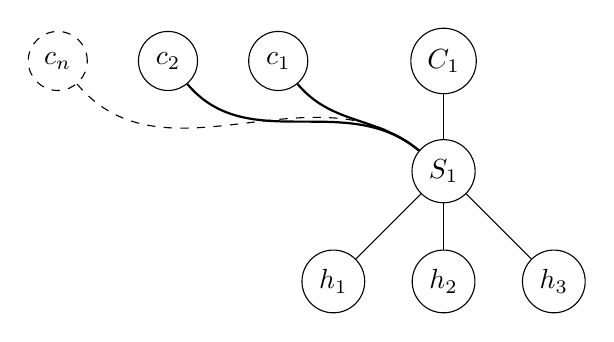
\begin{tikzpicture}[
      every node/.style={draw, circle, minimum width=0.75cm},
      x=0.7cm,
      y=0.7cm]
    \node (c1)    at (-3,  2) {$c_1$};
    \node (c2)    at (-5,  2) {$c_2$};
    \node [dashed] (cn) at (-7, 2) {$c_n$};

    \node (ctrl1) at ( 0,  2) {$C_1$};
    \node (S1)    at ( 0,  0) {$S_1$};
    \node (h1)    at (-2, -2) {$h_1$};
    \node (h2)    at ( 0, -2) {$h_2$};
    \node (h3)    at ( 2, -2) {$h_3$};

    \draw [thick] (c1) to[out=310,in=140] (S1);
    \draw [thick] (c2) to[out=310,in=140] (S1);
    \draw [dashed] (cn) to[out=310,in=140] (S1);

    \draw (S1) -- (ctrl1);
    \draw (S1) -- (h1);
    \draw (S1) -- (h2);
    \draw (S1) -- (h3);

  \end{tikzpicture}
  \caption{A single switch $S_1$ with its controller $C_1$, connected
    to end-hosts $h_1$, $h_2$, $h_3$ and clients $c_1$, $c_2$, $\dots$, $c_n$
    through ports.}
  \label{figure:graph.single.switch}
\end{figure}

The topology in figure \vref{figure:graph.single.switch} allows us to
program the controller to replicate client messages to all its hosts.
This is also called \textit{mirroring}\index{mirroring}.
%
We can do this by duplicating each incoming client packet,
forwarding packets with headers rewritten to match each
host's Ethernet and IP-address.  Duplicate replies to the clients should be
discarded, but we will ignore that for now.
%
The services will then process packets and---assuming the service protocol
is deterministic with regards to its input---end up in equal states.
%
While this should work well for \acs{UDP}\index{UDP!replication}, which is
stateless\index{stateless}, it would be \textit{significantly} more involved
for \acs{TCP}\index{TCP!replication}.  We discuss TCP replication in chapter
\vref{chapter:tcp.replication}.

However, a single switch is inherently prone to failure.  Should it fail, it
would take down all the services along with it.
%
The obvious step is to add more switches.
%
But adding a second switch will not be sufficient.  Should the two sets of
hosts end up in different states---in the case packet loss, for
example---they would not be able to decide whose state is correct.
%
We will therefore look at using three switches.

\begin{figure}[H]
  \centering
  \begin{tikzpicture}[every node/.style={draw, circle},x=0.7cm,y=0.7cm]
    \foreach \n in {1,2,3} {
      \pgfmathsetmacro\x{(\n-2)*6}
      \node (c\n)    at (\x - 2,  2) {$c_\n$};
      \node (ctrl\n) at (\x ,  2) {$C_\n$};
      \node (S\n)    at (\x ,  0) {$S_\n$};

      \draw (c\n) to[out=305,in=125] (S\n);
      \draw (S\n) -- (ctrl\n);

      \foreach \h in {1,2,3} {
        \pgfmathsetmacro\pos{(\h - 2)*2}
        \pgfmathtruncatemacro\num{((\n - 1)*3) + int(\h)}
        \node (h\num) at (\x + \pos, -2) {$h_{\num}$};
        \draw (S\n) -- (h\num);
      }

    }

    % Links between switches
    \draw (S1) to[out=-10,in=190] (S2);
    \draw (S2) to[out=-10,in=190] (S3);

    % Fail-over links
    % c1
    \node [draw=none] (c1up) [above of=c1] {};
    \draw [dashed] (c1) to[out=90,in=270] (c1up);

    % c2
    \node [draw=none] (c2up) [above of=c2] {};
    \draw [dashed] (c2) to[out=90,in=270] (c2up);

    % c3
    \node [draw=none] (c3up) [above of=c3] {};
    \draw [dashed] (c3) to[out=90,in=270] (c3up);

    % S1 -- S3
    \draw [dashed] (S1) to[out=-15,in=195] (S3);

  \end{tikzpicture}
  \caption{Three switches $S_1, S_2, S_3$ with controllers $C_1, C_2, C_3$ acting as Paxos nodes.
           The dashed line between $S_1$ and $S_3$ is a potential fail-over
             link.  Each client is assumed to be able to connect to any
             switch.}
  \label{figure:graph.three.switches}
\end{figure}

Figure \vref{figure:graph.three.switches} presents three interconnected
switches.
%
Potential fail-over links are indicated as dashed lines.  This is in case
a switch fails.  Again, we disregard the details concerning the fail-over
system for clients.

We still want to perform service replication using this topology, but now our
latencies are \textit{asymmetrical}:
%
Given equal link-latencies, a packet sent from $c_1$ to $h_9$ traverses more links than a packet from
$c_1$ to $h_1$.  The packets may therefore
arrive at different times at $h_1$ and $h_9$.
%
This causes an \textit{ordering problem}. If packets from several clients
reach hosts at different times, they will also arrive in different order.
This may break the service protocol or cause service states to differ.
%
To mitigate this problem, we need a mechanism to make sure that packets are
delivered \textit{in the same order}.
%
The switches should agree on some order---i.e., reach a \textit{consensus}.
In case of disagreements, we will let a majority decide---a
\textit{quorum}---and to form a quorum, we need at least three switches.

We have chosen the Paxos algorithm to resolve the ordering problem.

\begin{figure}[H]
  \centering
  \begin{tikzpicture}[every node/.style={draw, circle},x=0.7cm,y=0.7cm]

    % For each switch ...
    \foreach \n in {1,2,3} {
      \pgfmathsetmacro\x{(\n-2)*6}
      \node (ctrl\n) at (\x ,  2) {$C_\n$};
      \node (S\n)    at (\x ,  0) {$S_\n$};

      \draw (S\n) -- (ctrl\n);

      % For each host ...
      \foreach \h in {1,2,3} {
        \pgfmathsetmacro\pos{(\h - 2)*2}
        \pgfmathtruncatemacro\num{((\n - 1)*3) + int(\h)}

        % Host node
        \node (h\num) at (\x + \pos, -2) {$h_{\num}$};
        \draw (S\n) -- (h\num);

        % Paxos node
        \node [very thick] (P\num) at (\x + \pos, -3.75) {$P$};
        \draw [dashed] (h\num) -- (P\num);
      }
    }

    % Links between switches
    \draw (S1) to[out=-10,in=190] (S2);
    \draw (S2) to[out=-10,in=190] (S3);
    \draw [dashed] (S1) to[out=-15,in=195] (S3);

  \end{tikzpicture}
  \caption{Support for Paxos on the servers $h_1, \dots, h_3$ requires a
    copy of the Paxos code $P$ on each server.}
  \label{figure:paxos.on.servers}
\end{figure}

Figure \vref{figure:paxos.on.servers} shows an straight-forward way of deploying
Paxos as middleware software frameworks on the end-hosts.

First let us reiterate our aim: To provide replication of the services
running on the hosts $h_1--h_9$. We do this by duplicating each incoming
client packet and use Paxos to reach an agreement on the order in which they
should be delivered to each end-host.

This configuration is obviously severely simplified, far from actual,
application-level Paxos configurations.
%
Specifically, one would most likely
spread each kind of replicated service across each switch, so that, e.g.,
$h_1$, $h_4$ and $h_7$ replicated service $A$, using Paxos nodes
$P_A^1$ on $h_1$, $P_A^2$ on $h_4$, or one could have an additional Paxos
system on a higher level, and so on.
%
Still, figure \ref{figure:paxos.on.servers} is useful to highlight some
problems with some conventional Paxos deployments.

We have removed the clients from the current and following figures for
clarity.  We still assume that the switches receive and transmit packets to
an unknown number of clients.

Now, assuming that Paxos has been deployed as middleware software as shown
in figure \ref{figure:paxos.on.servers}, we can point out a few drawbacks
for this particular configuration:

\begin{itemize}
  \item \textbf{Application-level messaging:}
  Paxos messages between each node ($P$) begin and end at the
  application-level, and must traverse down the whole networking
  stack, over the links and back up again.
  %
  There is some inherent overhead in doing so, and for certain traffic
  patterns--when there are a lot of messages to transmit, e.g.---this
  \textit{could} become a problem for total system responsiveness.

  \item \textbf{Non-central network placement:}
  The Paxos nodes are positioned away from the central switching components
  of the network (i.e., the switches $S_1 \dots S_3$), requiring additional
  link-hops to reach their destinations.

  \item \textbf{Software requires built-in Paxos:}
  Finally, only software that that comes with Paxos built-in can possibly
  support it.  This can potentially become a problem for, e.g., businesses
  that unexpectedly need to scale a service---especially when considering
  services that run in the cloud.
\end{itemize}

Now consider the situation where the \textit{switch} (along with its
controller) provides Paxos capabilities\index{Paxos!on switch} (figure
\ref{figure:paxos.on.switches}).

\begin{figure}[H]
  \centering
  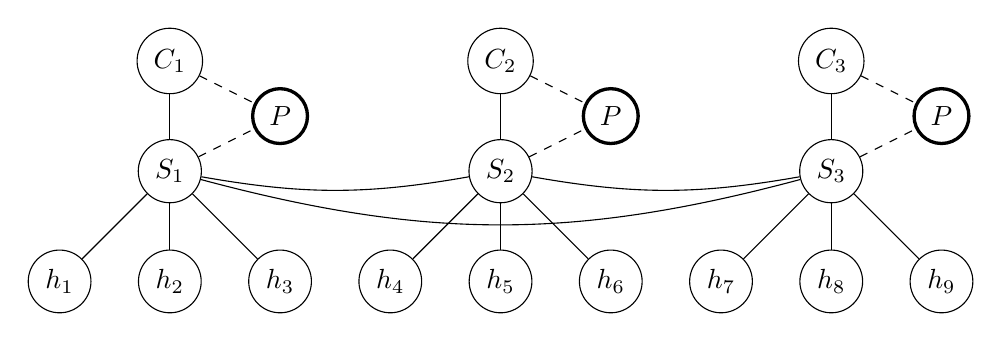
\begin{tikzpicture}[every node/.style={draw, circle},x=0.7cm,y=0.7cm]

    % For each switch ...
    \foreach \n in {1,2,3} {
      \pgfmathsetmacro\x{(\n-2)*6}
      \node (ctrl\n) at (\x ,  2) {$C_\n$};
      \node (S\n)    at (\x ,  0) {$S_\n$};

      \draw (S\n) -- (ctrl\n);

      % Paxos node
      \node [very thick] (P\n) at (\x + 2, 1) {$P$};
      \draw [dashed] (S\n) -- (P\n);
      \draw [dashed] (ctrl\n) -- (P\n);

      % For each host ...
      \foreach \h in {1,2,3} {
        \pgfmathsetmacro\pos{(\h - 2)*2}
        \pgfmathtruncatemacro\num{((\n - 1)*3) + int(\h)}

        % Host node
        \node (h\num) at (\x + \pos, -2) {$h_{\num}$};
        \draw (S\n) -- (h\num);
      }
    }

    % Links between switches
    \draw (S1) to[out=-10,in=190] (S2);
    \draw (S2) to[out=-10,in=190] (S3);
    \draw (S1) to[out=-15,in=195] (S3);

  \end{tikzpicture}
  \caption{Paxos ($P$) in the switches $S_1, S_2, S_3$ mitigates the need for special code on the servers.}
  \label{figure:paxos.on.switches}
\end{figure}

In figure \ref{figure:paxos.on.switches}, the switches themselves (and their
controllers\index{Paxos!controller}) enable
support for Paxos.\footnote{We have moved the servers to several switches
to indicate a distributed nature between the switches.
Paxos on a single switch would not be very useful, as that would be a single
point of failure and---after all---be the sole decision point for message
ordering.}
%
This should let the end-host services be oblivious to the fact that Paxos is
used to order the arrival of packets to them, providing Paxos
\textit{transparently}.

Besides, Paxos is now run at a much lower networking level\index{networking
levels} and at the point where switching is done---there will be fewer hops
for each packet.

Of course, this solution is neither without limitations:

\begin{itemize}
  \item \textbf{Must perform ordering on each packet:}

Performing Paxos ordering at the level of each packet means that a lot of
Paxos messages must be exchanged.  For networks with a small \ac{MTU}, a
large packet may be split up into several smaller ones.  Thus, the advantage
of switch-level Paxos may soon become a bottleneck in itself, especially
when client messages are large.

  \item \textbf{Cannot exploit application-level protocol:}

Also, at this level we lose opportunity of exploiting knowledge about
each client-server protocol.  As a hypothetical example, a server may know
that some client operations are side-effects free (a
\textit{read}-operation on a key-value server, for instance), and can
choose not to initiate a Paxos exchange for such operations.

  \item \textbf{Only supports deterministic services:}

And some service protocols simply do not fit into this model
of replication at all.  The obvious example is services that are not
deterministic on their input---meaning that if two identical services 
receive exactly the same input, in exactly the same order, their internal
states may become different.

\end{itemize}

But many services should still fit in to a model of switch-level
Paxos replication.  For instance, replicating a \acs{UDP}-based logging
server could prove to be beneficial.

We will not delve deeper into this matter.  Especially, we completely
disregard details concerning replies back to the clients: We silently
drop duplicated replies.  A deeper study would certainly take a closer
look at such situations, and we discuss a result regarding TCP in section
\ref{chapter:tcp.replication}.

Neither have we looked more at the situation when a switch goes down.
We have indicated fail-over links in the topologies, but have not
implemented such functionality.  For the part that concerns Paxos, such a
situation should start a new leader election.  If a switch comes back up
again, it should synchronize the state of its services with the others.
All of these are separate studies on their own, but we would like to note
that OpenFlow does have some support for monitoring link-status, and it
would be very interesting to make use of that in the face of failures.

Finally, we have not attempted to make an optimal design.  We concentrate
solely on the part of finding out if implementing Paxos on the switch-level
is \textit{possible} and if it could be \textit{useful}.

